\documentclass[10pt]{article}

% amsmath package, useful for mathematical formulas
\usepackage{amsmath}
% amssymb package, useful for mathematical symbols
\usepackage{amssymb}

% graphicx package, useful for including eps and pdf graphics
% include graphics with the command \includegraphics
\usepackage{graphicx}

% cite package, to clean up citations in the main text. Do not remove.
\usepackage{cite}

\usepackage{color} 

% Use doublespacing - comment out for single spacing
\usepackage{setspace} 
\doublespacing

% Text layout
\topmargin 0.0cm
\oddsidemargin 0.5cm
\evensidemargin 0.5cm
\textwidth 16cm 
\textheight 21cm

% Bold the 'Figure #' in the caption and separate it with a period
% Captions will be left justified
\usepackage[labelfont=bf,labelsep=period,justification=raggedright]{caption}

% Use the PLoS provided bibtex style
\bibliographystyle{plos2009}

% Remove brackets from numbering in List of References
\makeatletter
\renewcommand{\@biblabel}[1]{\quad#1.}
\makeatother


% Leave date blank
\date{}

\pagestyle{myheadings}
%% ** EDIT HERE **


%% ** EDIT HERE **
%% PLEASE INCLUDE ALL MACROS BELOW

% figure files reside in the figures/ directory
\graphicspath{
{figures/}
}

%% END MACROS SECTION

\begin{document}

% Title must be 150 characters or less
\begin{flushleft}
{\Large
\textbf{Title}
}
% Insert Author names, affiliations and corresponding author email.
\\
Author1$^{1}$, 
Author2$^{2}$, 
Author3$^{3,\ast}$
\\
\bf{1} Author1 Dept/Program/Center, Institution Name, City, State, Country
\\
\bf{2} Author2 Dept/Program/Center, Institution Name, City, State, Country
\\
\bf{3} Author3 Dept/Program/Center, Institution Name, City, State, Country
\\
$\ast$ E-mail: Corresponding author@institute.edu
\end{flushleft}

% Please keep the abstract between 250 and 300 words
\section*{Abstract}

% Please keep the Author Summary between 150 and 200 words
% Use first person. PLoS ONE authors please skip this step. 
% Author Summary not valid for PLoS ONE submissions.   
\section*{Author Summary}

\section*{Introduction}

The adaptive immune response induced during an acute viral infection is a complex web of defense mechanisms able to control all but the most virulent of infections.   A complete understanding of the evolution of this response will be instrumental in the design of antiviral prophylaxis, therapy and vaccine interventions.   The effector arm of the immune response operates, however, under strict constraints of time and the geography of body structure during the dynamic spread of replicating viruses.  Elegant studies have outlined the role of local dendritic cells in detecting invasion and delivering antigen-specific cargoes to the lymph nodes [1-3].  In situ imaging has provided temporal and spatial details on the communications between dendritic cells and recirculating precursor or memory T and B cells within the lymph node architecture [4-6].  The specificity, activation profile and functional capabilities of resulting effector lymphocytes are well described [7-9].  In contrast to the induction phase of the response, how activated lymphocytes emanating from regional lymph nodes efficiently ‘search’ for the infected tissue, often called the lymphocyte diaspora [10], has been less well studied. 

The immune response to influenza A virus (IAV) is arguably the most well-studied with respect to viral specificity, individual immunocyte components, whole animal models, and mathematical modeling.  Animal models of IAV include the non-human primate, ferret, and mouse [11].   Although not a natural host of influenza viruses, the inbred mouse model has provided a detailed description of viral and immunocyte dynamics.  Mathematical models have used the mouse model data to simulate the evolution of the immune response and its impact on viral kinetics [12-16].  These mathematical models have approached such questions as the relative roles of antibody and cytotoxic T lymphocytes (CTL), number of CTL required, regulation of antigen presentation, and comparing drug intervention strategies.  Such whole-response modeling has the potential advantage of selecting the most promising strategies of vaccination and therapy for subsequent expensive animal and human trials.   Each of these models, however, must make assumptions about the efficiency of each functional component in the model.   Math modeling can also inform us on the behavior of each component.

Here we approach the more focused problems of time and physical constraints on the lymphocyte diaspora.  How do very small foci of infected tissue attract limited numbers of activated CTL released into the systemic vascular system servicing non-infected tissue orders of magnitude larger than the target infection?  A host of chemokines secreted by infected cells, with signal amplification by immigrating inflammatory cells, are critical in directing inflammatory and immune cells to sites of inflammation [17-19].  While each chemokine has been studied in detail for its synthesis, receptor specificity and function in knockout models, the spatial and temporal details of chemokine function and efficiency have not been explicitly modeled in a virus-infected whole animal environment.

Using an agent-based model (ABM) designed to test the temporal and spatial demands during an acute influenza infection in the lung, we examined the homing of CTL to infected foci in the lung and how chemokines secreted by infected epithelial cells contributed to infection control.   Viral secretion dynamics and detailed chemokine secretion patterns by infected human epithelial cells in vitro [20] provided the data representing local behaviors at the alveolar level.  Data on CTL production and recirculation and the resolution of viral infections was obtained from the literature on mouse infections.   We excluded the role of immigrating inflammatory cells in order to focus on the contribution of two chemokines induced during infection with three influenza viruses, including a seasonal H1N1 virus, the pandemic H1N1 virus, and a virulent avian H5N1 virus.  In our modeling environment we observed the markedly different efficiencies of control for the three influenza viruses, differing effectiveness of the two chemokines, and the importance of the velocity of CTL search within tissue.

% You may title this section "Methods" or "Models". 
% "Models" is not a valid title for PLoS ONE authors. However, PLoS ONE
% authors may use "Analysis" 
\section*{Models}

\subsection*{Computational Modeling}

\begin{figure}[ht!]
\begin{center}
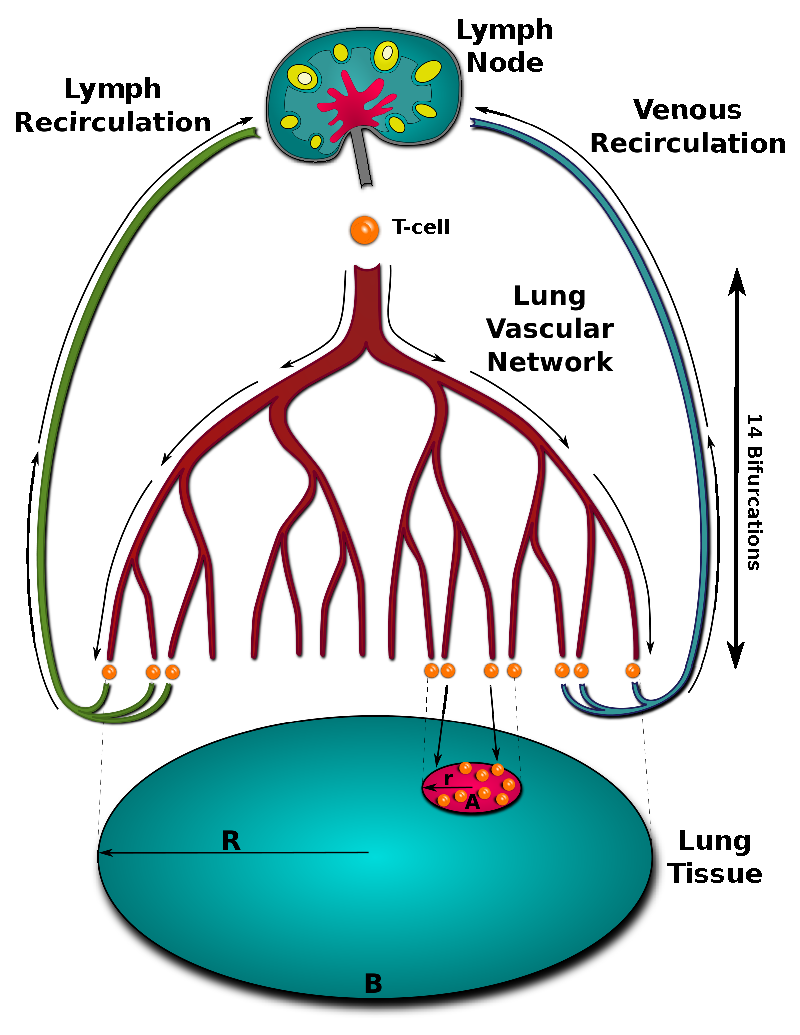
\includegraphics[width=0.4\textwidth]{SystemChart}
\end{center}
\caption{A region of infected tissue of radius $r$ (shaded region $A$) expressing chemokines and inflammatory signals. This region is surrounded by region $B$ which does not have any infected cells and hence does not express either chemokines or inflammatory signals. The $2^{14}$ capillaries (red circles) are distributed evenly throughout the entire lung (region $A$ and $B$).}
\label{fig:systemchart}
\end{figure}

% FIXME: The main goal of this paper is to compare chemokine signaling effectiveness between infections from different strains of influenza. Our study looks at separate infections from three different strains: seasonal, avian, and swine. Futhermore, we compare the roles of two established signaling molecules: CXCL10 (IP-10) and CCL5 (RANTES).

FIXME: Need to say somewhere that we simulate a generic chemokinetic signal that abstracts X, Y, and Z.

Computational modeling was conducted using Cycells [REFERENCE], a modeling platform for implementing two- or three-dimensional agent-based simulations of immune response [CITATIONS].
%developed for studying the spread of influenza and tuberculosis in tissue [CITATIONS].
%
%It has an interface for defining cell types and molecules. For example, the T cell type can be defined as having a particular size, lifespan, movement rate, change in state in response to contacting a DC or change in motion in response to contacting a chemokine. Cycells will be modified to account for flows between lymph nodes, the circulatory system and tissue compartments.
A simplified model of T-Cell activation and recirculation was implemented in Cycells (Fig 1), and simulations were conducted to measure efficiency of infection clearance under different environmental conditions. To model a growing infection, the lung was represented as a two dimensional sheet of healthy eptithelial cells. Vasculature was represented as a binary tree with fourteen branches originating at a single lymph node. Activated T-cells descend through the vascular tree until chemotactic signal is detected, at which point they exit the vasculature and follow the [FIXME chemokine/inflammatory] gradient to the site of infection. T-cells that do not encounter chemokine recirculate to the lymph node. Once at the site of infection, a T-Cell may encounter an infected epithelial cell and induce apoptosis.

The simulation begins when a single cell in the center of the tissue is infected. After the eclipse phase (incubation), the infected cell begins secreting virus and chemokine. Virus diffuses locally, infecting nearby cells, and continuing the cycle. The chemokine diffuses from secreting cells, thus increasing the size of the signaling area. After a delay, to simulate lymph node stimulation and T-Cell proliferation, activated T-cells begin exiting the lymph node and circulating through the vasculature to the tissue. Because T-Cells cannot choose their path through the branching network, we assume they arrive in tissue at random locations. Figure \ref{fig:modelchart} illustrates the model components 
(epithelial cells, T-cells, and particles) and how they transition between different states.

\subsection*{Model Definition}

\begin{figure}[ht!]
\begin{center}
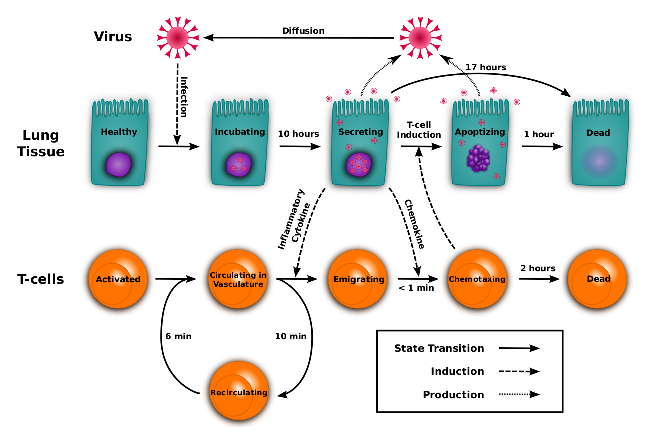
\includegraphics[width=\textwidth]{ModelChart}
\end{center}
\caption{Computational model: Components and state transitions.}
\label{fig:modelchart}
\end{figure}

Epithelial cells are stationary and can be in of five different states: \emph{healthy}, \emph{infected}, \emph{expressing}, \emph{apoptotic}, and \emph{dead}. Healthy cells remain unchanged unless infected by virus. Once infected, there is a 10h incubation window before the cell transitions to \emph{expressing}. \emph{Expressing} cells secrete virus and chemokine for 17 hours when they die. \emph{Expressing} cells become \emph{apoptotic} if they encounter activated T-cells. Apoptosising cells continue to secrete virus and die one hour after their transition. \emph{Dead} cells remain inert and do not regenerate over the course of an infection.

T-cells have three states: \emph{Searching}, \emph{Recirculating}, and \emph{Activated}. T-Cells begin emerging from the lymph node at five days post infection and continue at the rate of 777 T-cells per hour for the duration of the simulation. T-Cells enter the vascular system in the \emph{Searching} state, arriving at a random location on the lung's surface. \emph{Searching} cells perform a random walk in the tissue for 10 minutes, after which they transition to \emph{Circulating} if they fail to encounter chemokine. Circulating cells spend six minutes recirculating to the lymph node where they are converted to \emph{Searching} and reintroduced to a new random location in the lung. If a \emph{Searching} T-Cell encounters chemokine, it immedaiately converts to \emph{Activated} and begins climbing the chemotactic gradient to the source of infection. \emph{Activated} T-Cells move continuously up the gradient and if they encounter \emph{Expressing} epithelial cells, the epithelial cell transitions \emph{apotosis}. Activated T-Cells decay exponentially with an average lifespan of two hours. FIXME-DREW[What happens after they decay? Is there a threshold after which they die or what?]

The model contains two kinds of particles: virus and chemokine. Both are produced at constant rates by \emph{Expressing} epithelial cells.
%As particles, both have their kinetics limited to diffusion and decay.
Virus diffuses through the lung tissue, infecting healthy cells probabilistically according to the local virus concentration. Chemokine diffuses across the tissue but has no
direct effect beyond activating T-Cells. Both particle types decay over time.
%purpose other than to activate searching T-cells.
FIXME-DREW[Viruses decay over time. Do Chemokines?]

\subsection*{Parameters}

Define CyCells environment.  Talk about the need for spatial model.  Human/mouse scaling.  Parameter definitions. 

\begin{table}
\begin{tabular}{ | c | c | c | }
  \hline                        
  Paramter & Value & Source \\
  \hline
  Viral Diffusion & .0318 & Stokes-Einstein / Beau \\
  Viral Decay &  1/day & Soumya \\
  Chemokine Diffusion & .318 & Stokes-Einstein \\
  Chemokine Decay &  3.8508e-4/s & 30m half-life \\
  Infection Sensitivity &  2h/virion & [1] \\
  Incubation Time &  10h & Mitchell \\
  Expression Time &  16.7h & Mitchell \\
  Apoptosis Time & 1h & Fred \\
  T-Cell Production Rate & 777/h & Soumya, Miao fits \\ 
  Circulation Time & 6m & Fred, mouse model \\
  Search Time & 10m & Fred, mouse model \\
  T-Cell Speed (Search) & $30 \mu m/s$ & Fred ? \\
  T-Cell Speed (Activated) & $3 \mu m/s$ & Fred ?\\
  T-Cell Sensitivity & $100 ng/ml$ & See Results \\
  T-Cell Expected Kill Rate & 10m & Fred/Drew \\
  Cell Radius & $25 \mu m$ & Fred \\
  T-Cell Age (Active) & 2h & Fred \\
  T-Cell Age (Other) & 3d & Fred \\
  T-Cell Ramp Up Time & 5d & Icaris \\
  IgM Strength & Viral decay of 3/day after day 3 & Soumya [3] \\
  \hline  
\end{tabular}
\caption{caption.}
\label{table:parameters}
\end{table}

\begin{table}
\begin{tabular}{ | c | c | c | }
  \hline                        
  Paramter & Value & Source \\
  \hline
  Chemokine Production Rate &  9.348e-5 (varies by strain) & [2] \\
  Virus Production Rate &  3.783e-4 (varies by strain) & Mitchell \\
  \hline  
\end{tabular}
\caption{Strain specific parameters}
\label{table:strains}
\end{table}

\begin{itemize}
\item[1] The molecular concentration where there is one molecule per eptithelial cell volume is 1.53e-17 mol/ml.  Thus, if you multiply the local viral concentration by 9.05e12 you get an infection event after two hours given that concentration.  This probability scales linearly with the viral concentration.
\item[2] These are calculated off of Fred's new data sets using the Mitchell ODE model and parameters as a basis.
\item[3] IgM is represented by increasing the viral decay rate to 3/day after the third day of the simulation.
\end{itemize}


% Results and Discussion can be combined.
\section*{Results}

\subsection*{Chemokine production}

Chemokine data was collected in conjunction with the Mitchell et al (REF) (Fig.~\ref{fig:data}).   Increases in IP-10 concentration are observed starting no later than eight hours post-infection and increases in RANTES concentration are seen no later than 16 hours post-infection.  We extended the ODE model established in Mitchell to allow for chemokine production from infected cells.  A genetic algorithm was used to find per cell production rates for both IP-10 and RANTES for the three different strains of influenza.  The production values for IP-10 are 7.15e-5 ng/cell*s for Avian, 9.35e-5 ng/cell*s for Seasonal, and 6.23e-5 ng/cell*s for Swine.  The values for RANTES are 3.90e-5 ng/cell*s for Avian, 1.27e-6 ng/cell*s for Seasonal, and 1.39e-6 ng/cell*s for Swine.  We observe consistent production values of each chemokine across the different strains with an exception of a larger production rate of RANTES in avian H5N1.  There seems to be no correlation between viral production and induced chemokine production across strains of influenza.

\begin{figure}[ht!]
\begin{center}
 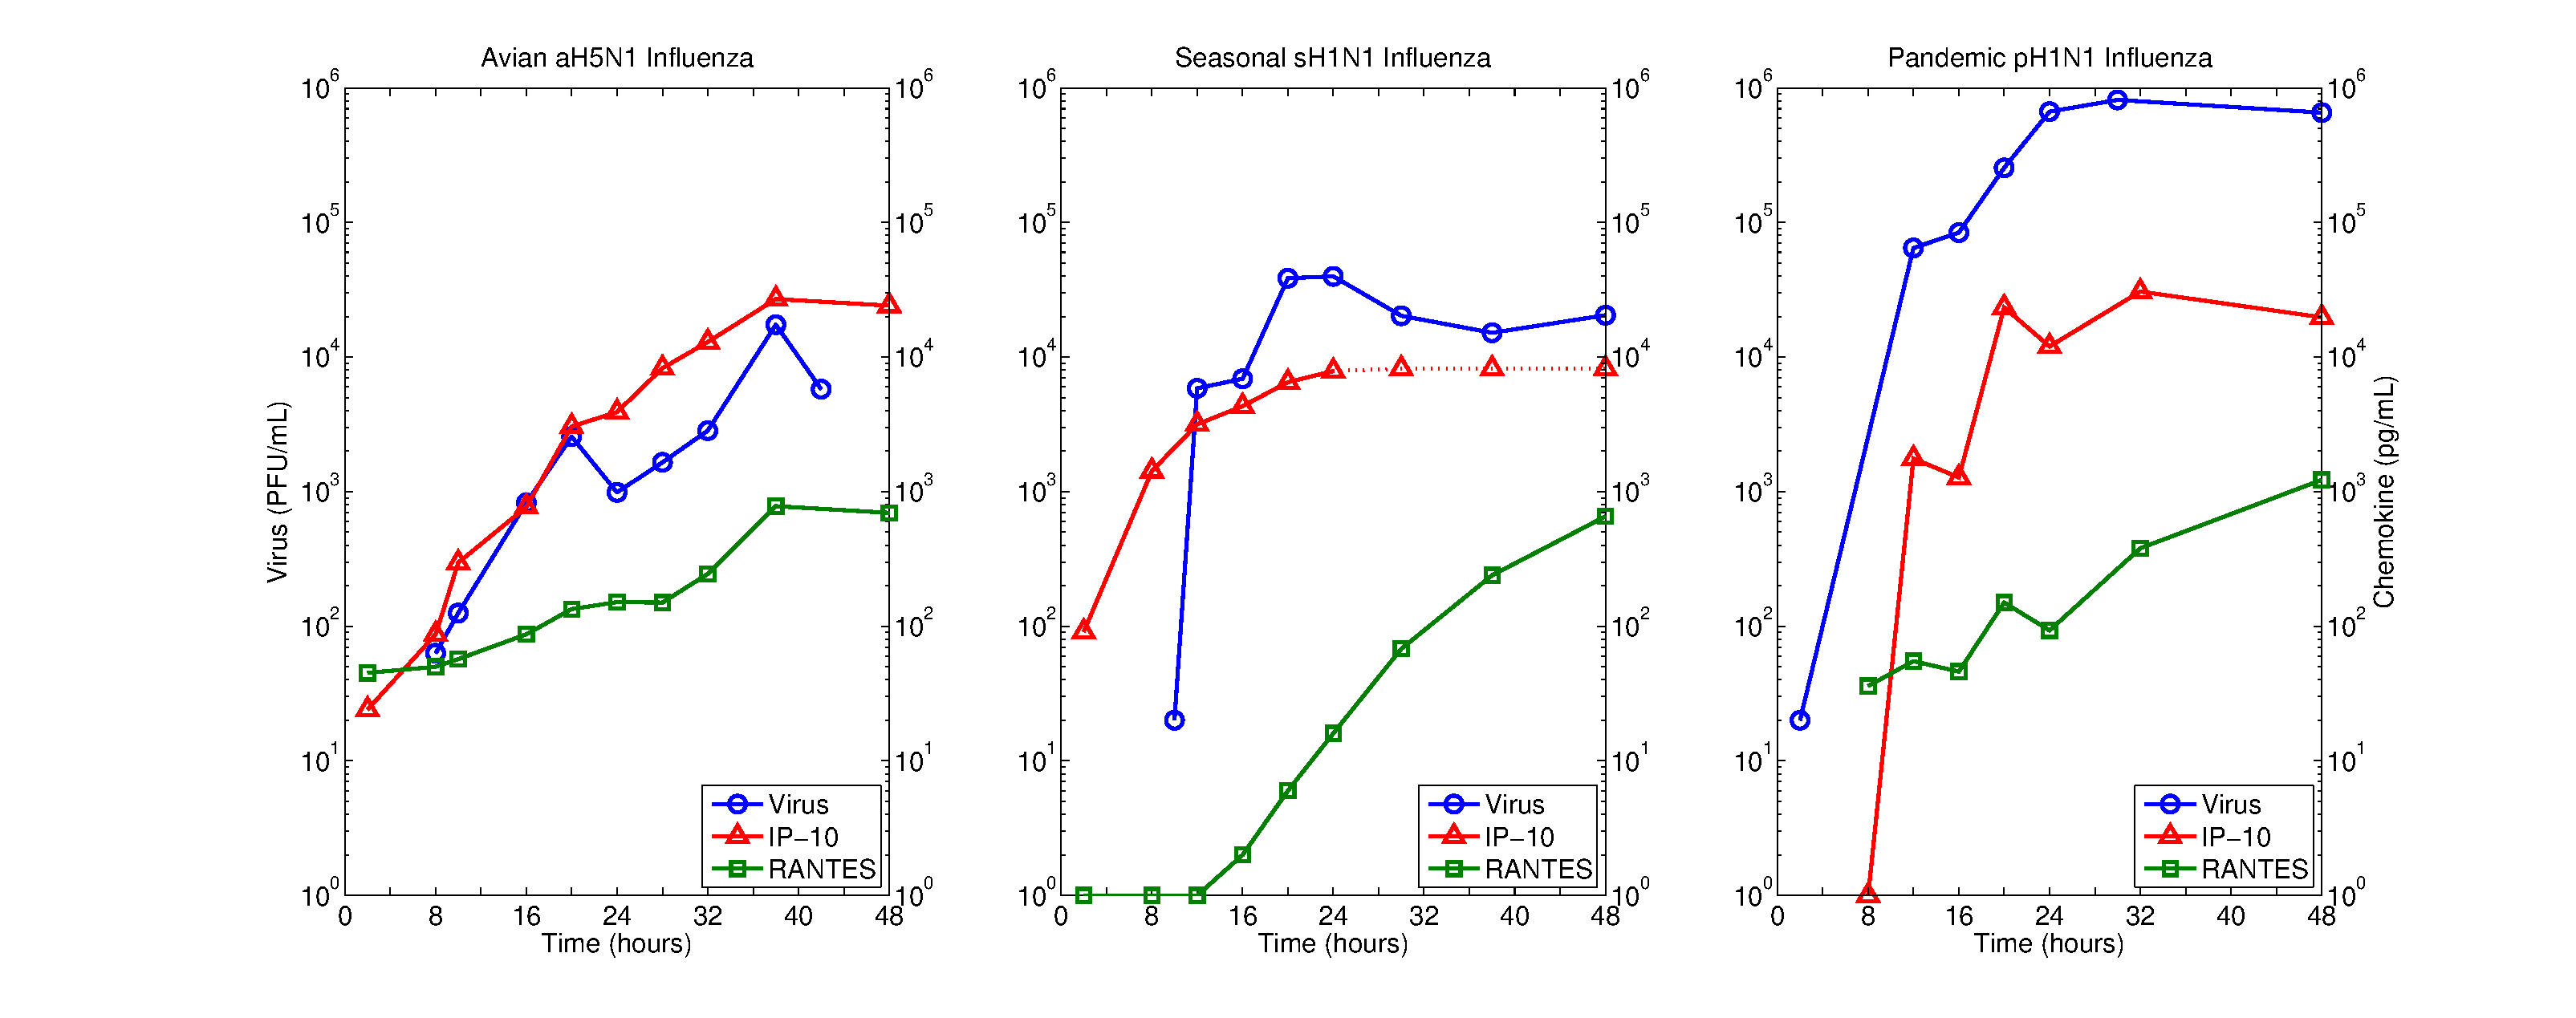
\includegraphics[width=.9\textwidth]{data}
 \end{center}
\caption{Empirical data of viral and cytokine titer for three strains of influenza: Avian H5N1 (A), Seasonal sH1N1 (B), and Pandemic pH1N1 (C).  For each strain, the viral load (blue circle) is shown in PFU/ml and the chemokines IP-10 (red triangle) and RANTES (green square) are shown in ng/ml.} 
 \label{fig:data}
\end{figure}

\subsection*{Model variance}

The parameters of the agent-based model are listed in Table~\ref{table:parameters}.  The model was run using calculated values of viral production and chemokine production for the three different strains of influenza.  To measure the variance of the stochastic model, we ran each model ten times using the default parameters (Fig.~\ref{fig:variance}).  The amount of variance between each run was calculated to be X .  The plots show total number of incubating, virus secreting, and apoptotic cells, but do not include dead cells.  Thus the figures approximate the rate of growth of the plaque over time.

Overlaying multiple runs reveals a slight elbow at day three of the infection.  This shift in the growth rate is due to the introduction of IgM antibodies that clear free virus.  Each infection shows a sharp decrease in infected cells at day five due to the T-cell response. 

\begin{figure}[ht!]
\begin{center}
 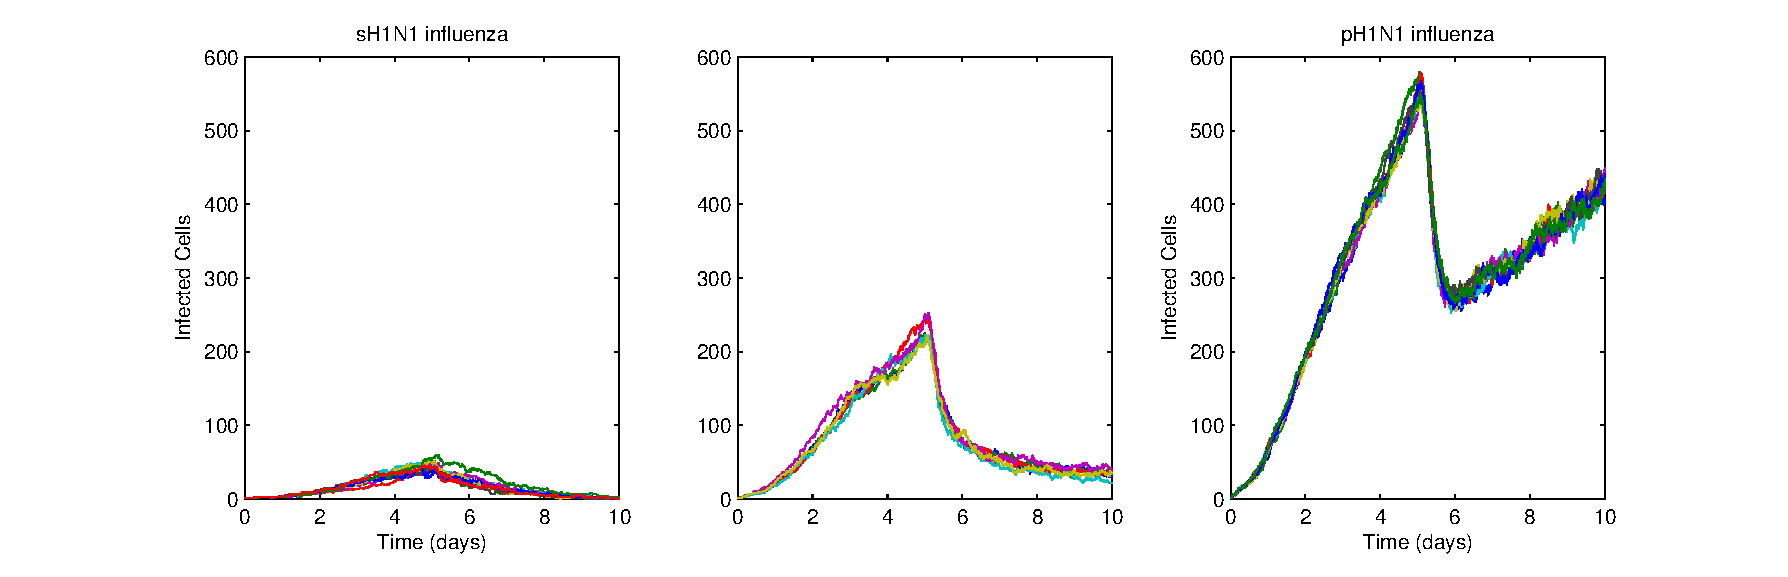
\includegraphics[width=\textwidth]{variance}
 \end{center}
\caption{Time series plots of ten runs of aH5N1 (A), sH1N1 (B), and pH1N1 (C) infections.  Both chemokines were used with the exception of aH5N1 which only produced RANTES.  The ten runs were initialized with the same parameters for each strain.  Plots show the number of infected, expressing, and apoptotic cells.  Dead cells are not included.  Variance arises from the stochastic nature of the agent-based model.  All three simulations are dramatically affected by the T-cell response at day five.  Each simulation uses a T-cell sensitivity to chemokine value of 1e-22.} 
 \label{fig:variance}
\end{figure}


\subsection*{Spatial effects}

Spatial effects of viral and chemokine diffusion play an important role in both the spread and the clearance of the infection.  Free virus particles diffuse from virus secreting cells and infect healthy cells.  Chemokine is also produced by infected cells and serves as chemotactic gradient for T-cells to follow to cells secreting virus.  Although virus is produced at a higher rate, it diffuses much more slowly than the two chemokines because it is a larger particle.  On the other hand, the chemokines are limited in their diffusion by a higher decay rate than virus.  This gives the two particle types similar spatial profiles (Fig.~\ref{fig:cycells}).

At day four, expressing cells make up a significant proportion of the infection and the total number of dead cells is relatively small.  By day seven, most expressing cells have been killed off by T-cells and most of the plaque consists of dead cells.  Furthermore, the pockets of concentrated chemokine lags somewhat behind the cell and virus spatial layout.  It takes time for newly secreting cells to produce chemokine and for old pockets of chemokine to decay away.  Thus, T-cells, which rely on the chemokine gradient to find infected cells, will often lag slightly behind the changes in the plaque.  The delayed response and the low proportion of virus secreting cells make it difficult for T-cells alone to completely clear the infection.

FROM FIGURE~\ref{fig:plaquesize} CAPTION: Early during the infection the plaque is dominated by cells that are active in producing more virus (incubating cells and secreting cells).  As the infection grows, cells in the middle of the plaque die and these active cells make up a decreasing proportion of the total size. At day five T-cells arrive and begin to kill any virus secreting cells they can find.  Initially, secreting cells make up a significant proportion of the total active cell population, but by day six the number of expressing cells has been reduced dramatically.   The H5N1 plaque is concentrated enough that the secreting cells can be found and completely eliminated.  On the other hand, both H1N1 simulations secreting cells are not completely eliminated.  These cells only account for at most 10\% of the active cell population and less than  1\% of the total plaque by day six.  T-cells continue to accumulate at the site of infection, but arrive at a slower rate than the plaque's rate of growth.  Because of this, it becomes more and more difficult for T-cells to find and kill the remaining expressing cells in order to shut down the infection.  Thus, the infection is able to recover and resume growth. 

\begin{figure}[ht!]
\begin{center}
 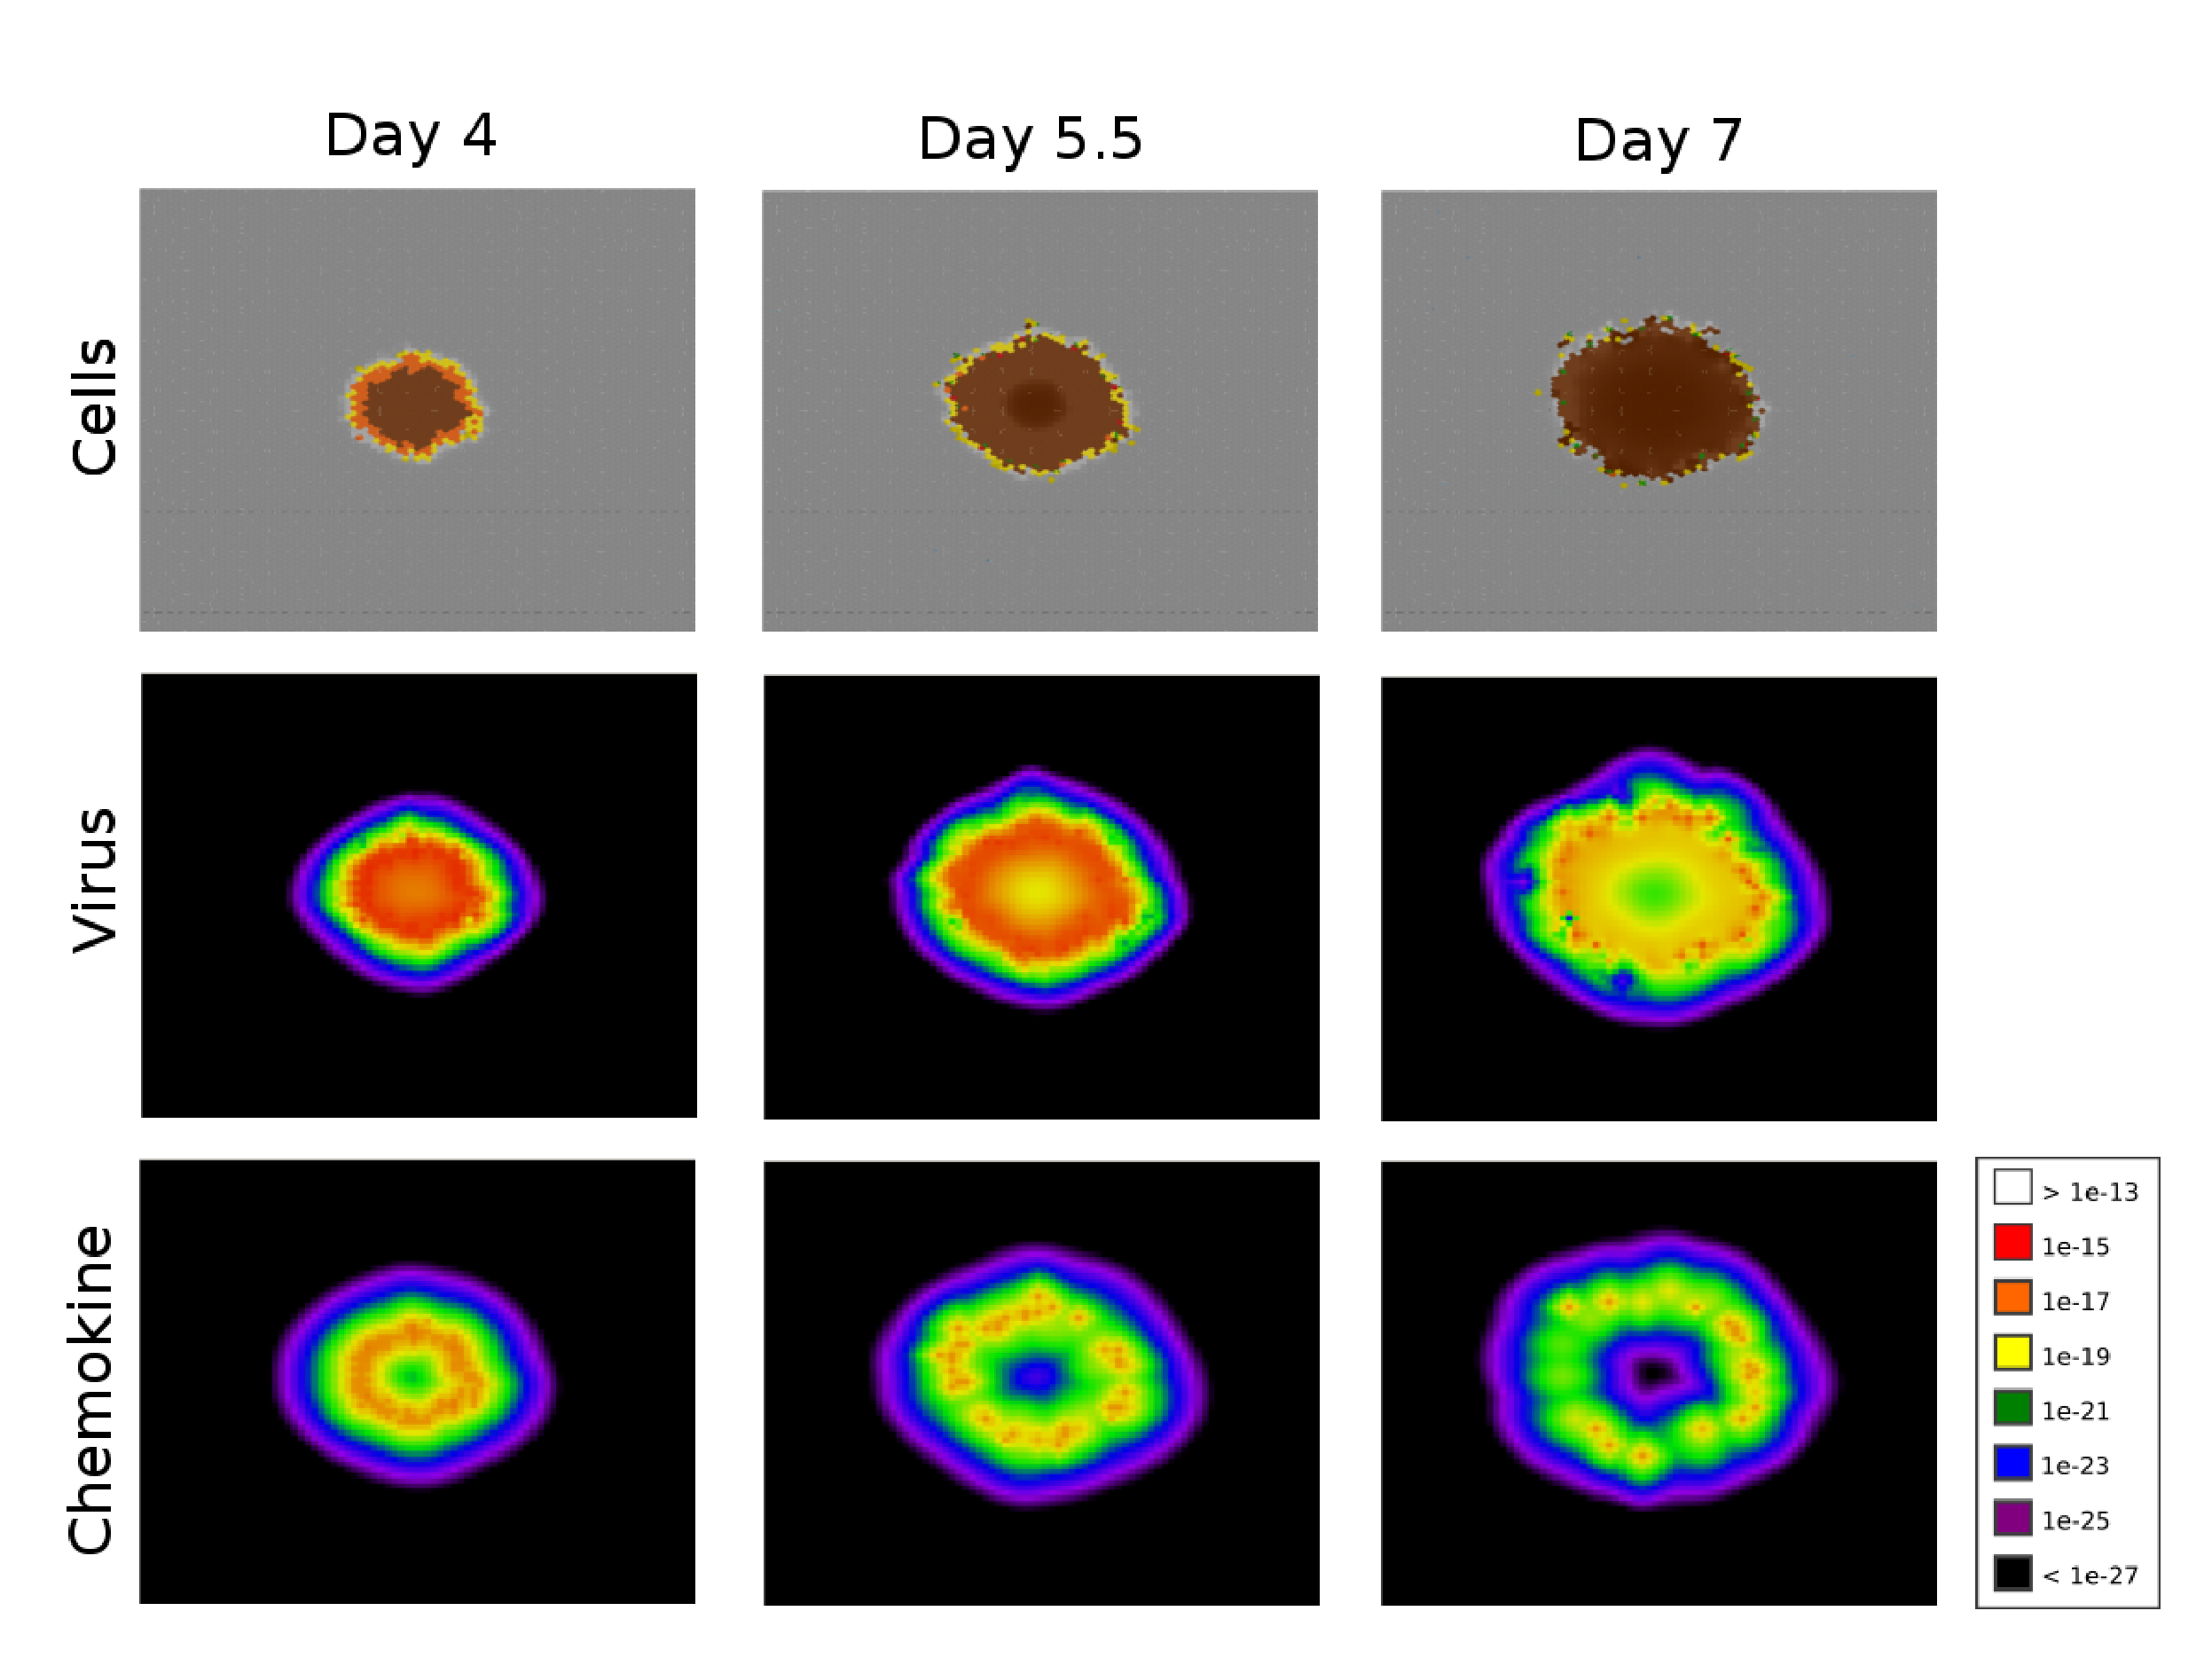
\includegraphics[width=\textwidth]{cycells}
 \end{center}
\caption{Screenshots taken at Day 4, Day 5.5, and Day 7 of a sample simulated sH1N1 infection.  The top row shows the spreading focus of infection  through the color coding of individual cells:  healthy cells in uninfected tissue (gray),  virus-incubating cells (yellow), virus-secreting cells (orange), apoptotic cells (red), dead cells (brown), and T-cells introduced at day 5 (green).  Free virus and chemokine particles are represented by compartmentalized concentrations of mols/ml and ng/ml (see the legend in the bottom right).  Each plot of virus and chemokine corresponds directly with the simultaneous cell figures.} 
 \label{fig:cycells}
\end{figure}



\subsection*{Infection dynamics}

The three strains show markedly different levels of virulence consistent with the results found in Mitchell (Fig.~\ref{fig:variance}).  Furthermore, the pandemic H1N1 grows so fast that the immune response is not able to contain the infection.  By the time the T-Cells arrive at the site of infection the plaque has become so spread out that the T-Cells are unable to cover the entire area.  Because H1N1 is produced at such a high rate, the window of opportunity for the T-Cells to stay ahead of the infection is too small (see discussion).  H5N1 is cleared completely, sH1N1 is contained but not fully cleared, and pH5N1 eventually recovers and continues to grow.  

ADD IP-10 RANTES COMPARISON

\subsection*{T-cell sensitivity to chemokine}

T-Cells exit a capillary when they can sense an inflammatory cytokine signal.  T-Cells then encounter a second signal, the chemokine gradient.  We use the chemokine gradient as an approximation of the inflammatory signal.  As seen in Figure \ref{fig:cycells}, chemokine is concentrated around virus secreting cells.  The threshold sensitivity level determines the minimum concentration of aggregate chemokine signal required for T-cells to detect the gradient.

To test what concentration the cytokine/chemokine signal is enough to recruit T-Cells from the capillaries we examined sensitivity levels that spanned seven orders of magnitude.  There is a threshold (Fig.~\ref{fig:sensitivity}) between the concentrations of (FIXME: new values) 1e-18 and 1e-19 (1e-19 and 1e-20 for pH1N1) after which there is no discernible difference in the infection kinetics.  Because multiple T-cells in the same area do not increase the rate of induction of apoptosis (killing), we hypothesize that there is a critical number of T-cells required to clear an infection after which there is no benefit gained from increasing numbers.  For consistency, all model runs were preformed using a sensitivity level of 1e-22.

NOTE TO SELF: Discuss the threshold in the discussion?  How does this threshold translate into a level of chemokine needed?  

\begin{figure}[ht!]
\begin{center}
 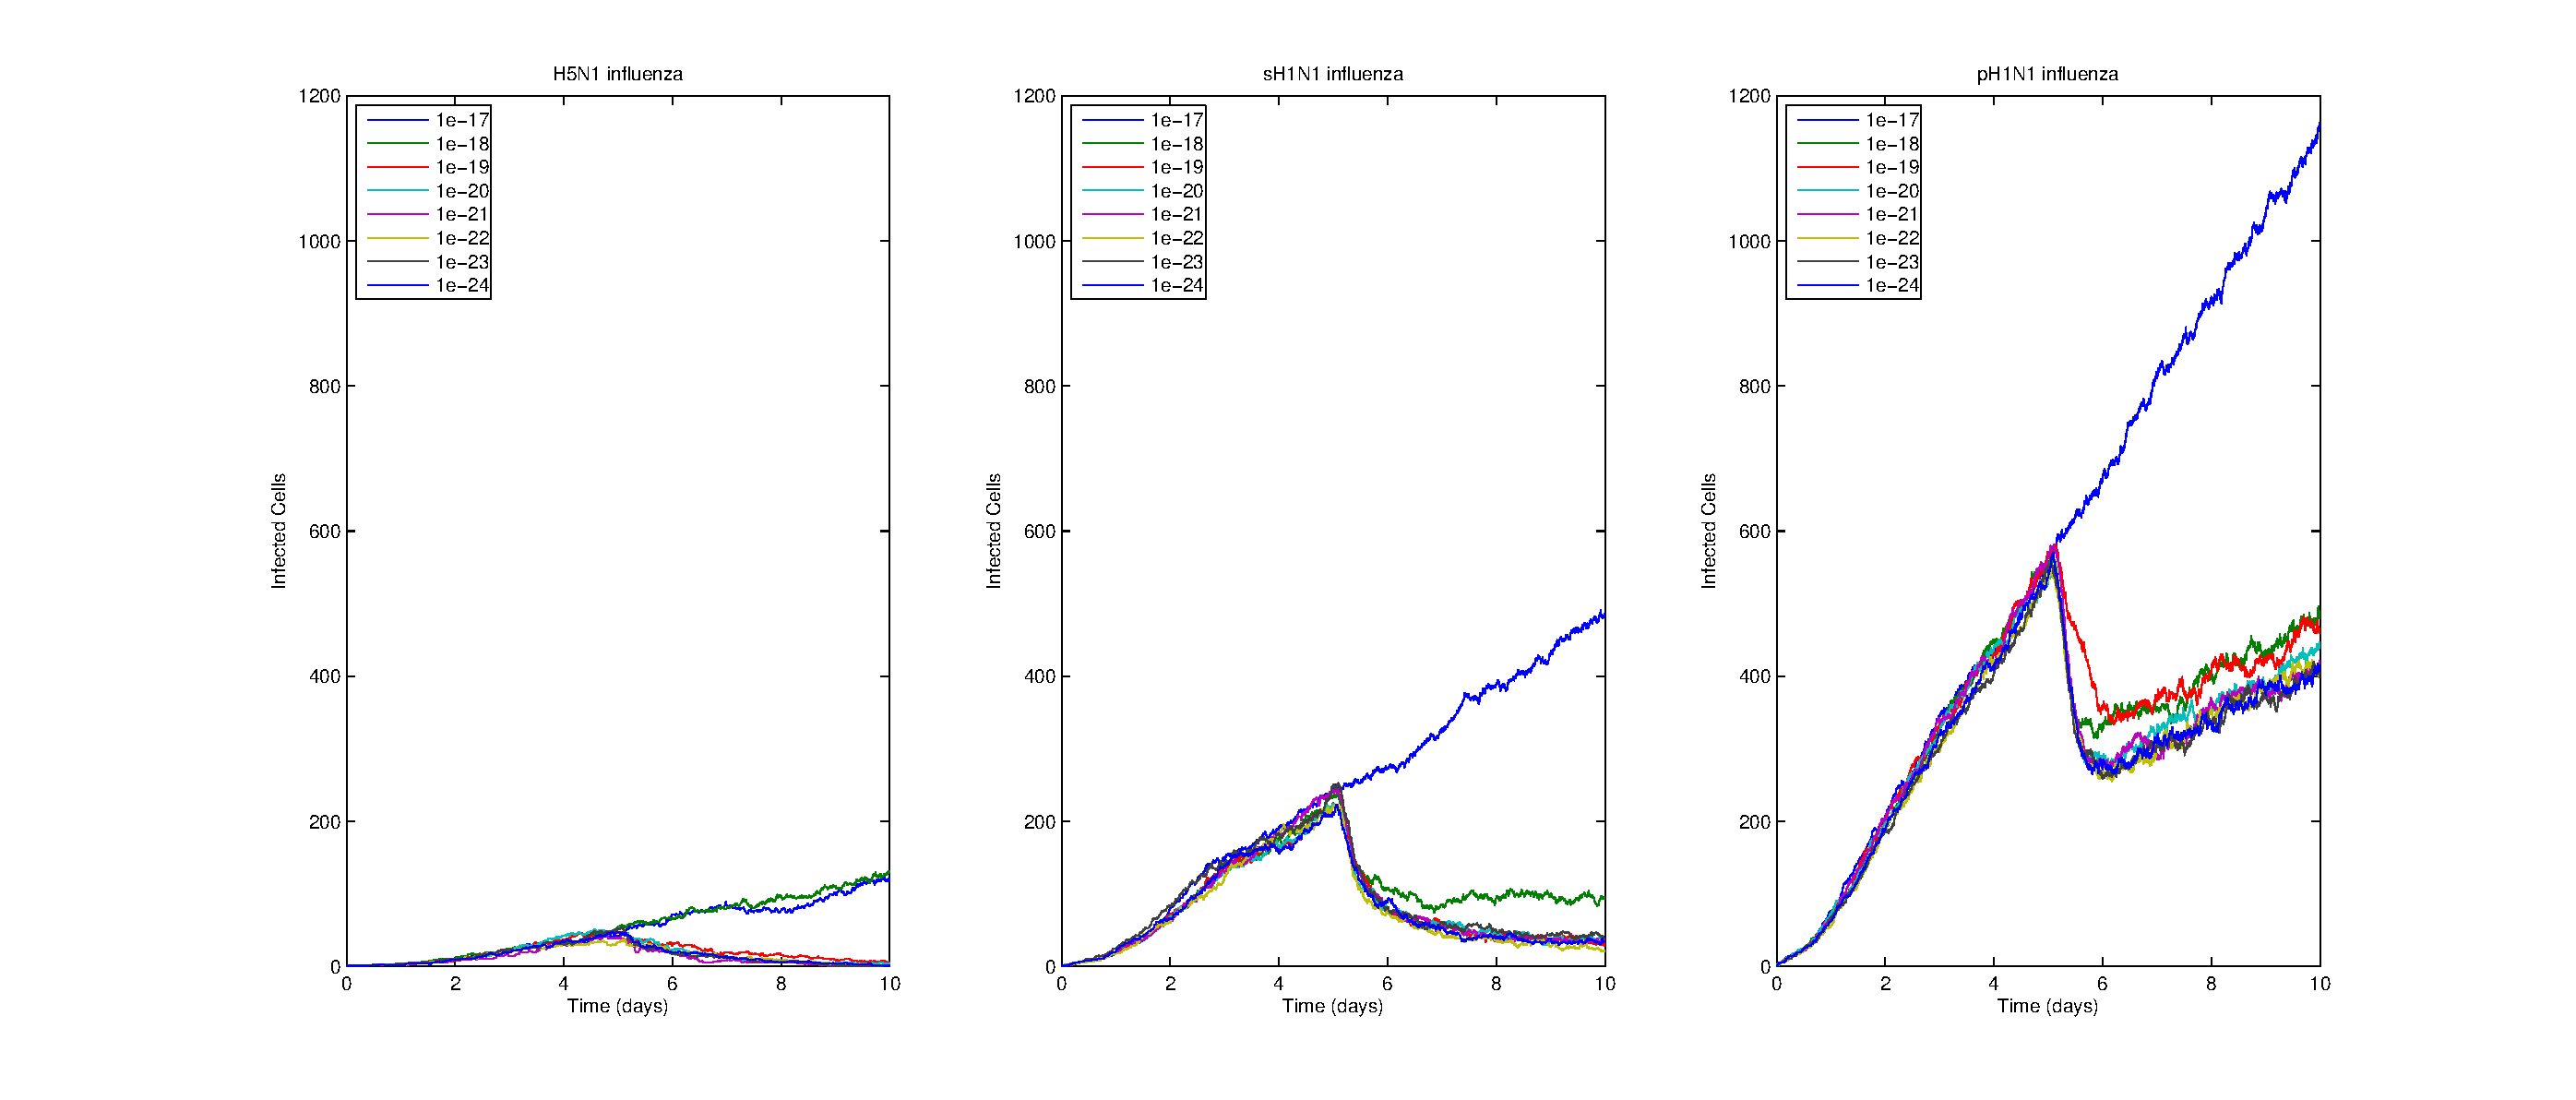
\includegraphics[width=\textwidth]{sensitivity}
 \end{center}
\caption{Plots of H5N1 using only RANTES and sH1N1 and pH1N1 infections using both IP-10 and RANTES with varying values for T-cell sensitivity to chemokine.  The plots show the total number of infected, expressing, and apoptotic cells for each infection.  The sensitivity value specifies the minimum level of chemokine concentration required for T-cells to detect it.  We notice a threshold between concentrations of 1e-18 and 1e-19 for H5N1 and sH1N1 and a threshold between 1e-19 and 1e-20 (NOTE TO SELF: 1e-21???) for pH1N1, after which there is no discernible difference in the infection kinetics.} 
 \label{fig:sensitivity}
\end{figure}

\subsection*{Infection resurgence}

As seen in Figure \ref{fig:variance}, the immune response fails to completely clear the seasonal infection and is unable to contain the pandemic infection.  We suggest this is an artifact of the spatial nature of the ABM.  Why can the immune response create an immediate decrease in the number of infected cells of the pandemic infection, only to fail in the same endeavor two days later?  It is important to note that Figure \ref{fig:variance} shows only the number of infected cells and does not include the number of dead cells in the focus of infection (FOI).  Furthermore, T-Cells are only able to induce apoptosis for epithelial cells that are presenting viral peptides.  This means that they do not kill incubating cells that are not yet expressing the virus.  At day 5.5, the proportion of expressing cells to the size of the FOI is high (Fig.~\ref{fig:cycells}).  By day seven however, the number of sH1N1 virus-secreting cells has decreased to a small fraction of the overall FOI size, whereas pH1N1 secreting cells remain a significant proportion of plaque size.  Even though the number of T-Cells at the site of infection continue to increase, the size of the plaque increases at an even faster rate.  Thus, the few remaining expressing cells become dilute, decreasing the efficiency of the T-cell search.  

By day seven the ratio of plaque size to the number of virus-secreting cells is approximately 100:1 for both the pH1N1 and sH1N1 strains.  However the greater replication rate of pH1N1 widens the gap between plaque size and fixed T-cell input (Fig.~\ref{plaquesize}C) whereas the lower replication rate of sH1N1 allows a match to T-cell input after day seven and subsequent control (but not elimination) of the sH1N1 infection.

A cell infected with pandemic influenza will produce new virus at the rate of 5.08e-3 particles/s.  This means that it will produce a new viral particle approximately every 200 seconds.  Assuming that virus particle secretion continues for one hour after apoptosis is initiated, the BEST a T-Cell can do is to limit a single infected cell to producing 18 new viral particles.  Thus, with no help from other immune sources, it becomes an impossible task for T-Cells alone to contain the pH1N1 infection.  In contrast, the sH1N1 virus-secreting cell produces a new virus particle every 2,643 seconds, so the T-cell can limit a single infected cell to produce only 1.3 viral particles in the one hour interval.  The avian virus-secreting cell will produce only 0.2 viral particles in the interval after T-cell detection. 


\begin{figure}[ht!]
\begin{center}
 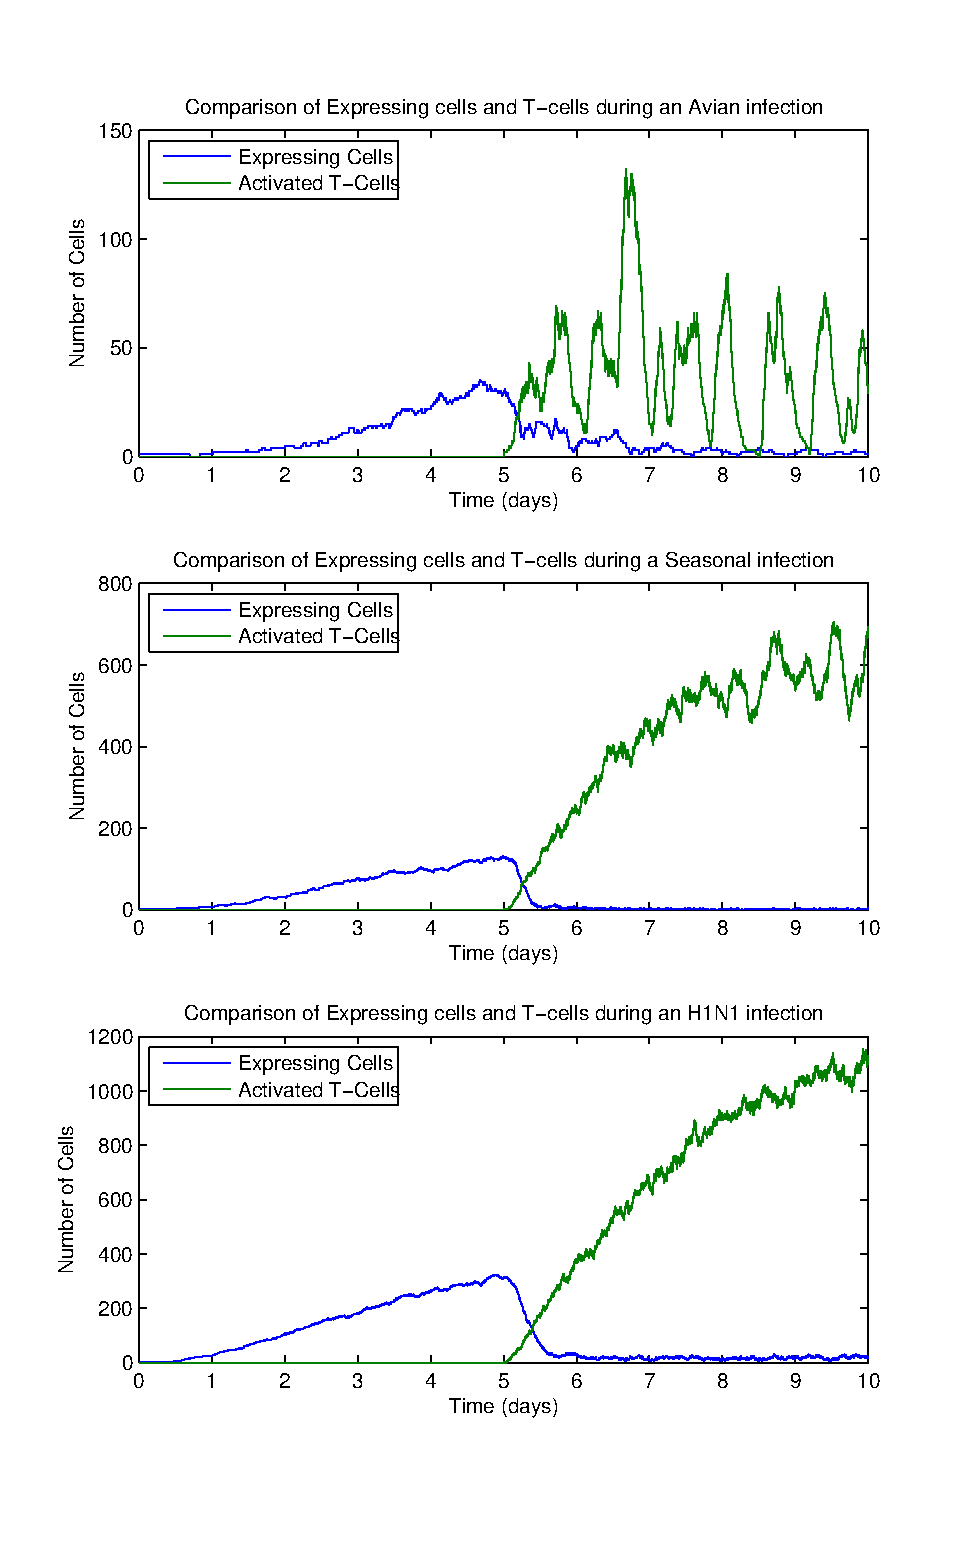
\includegraphics[width=0.7\textwidth]{searcharea}
 \end{center}
\caption{Comparison of the number of T-cells at the site of infection and the number of expressing cells left in the plaque.  Although T-cell counts continue to increase, the number of expressing cells the T-cells are targeting become fewer and far between.  By day six, an equilibrium is reached where T-cells are only able to contain (and not clear) the remaining expressing cells. } 
 \label{fig:searcharea}
\end{figure}


\begin{figure}[ht!]
\begin{center}
 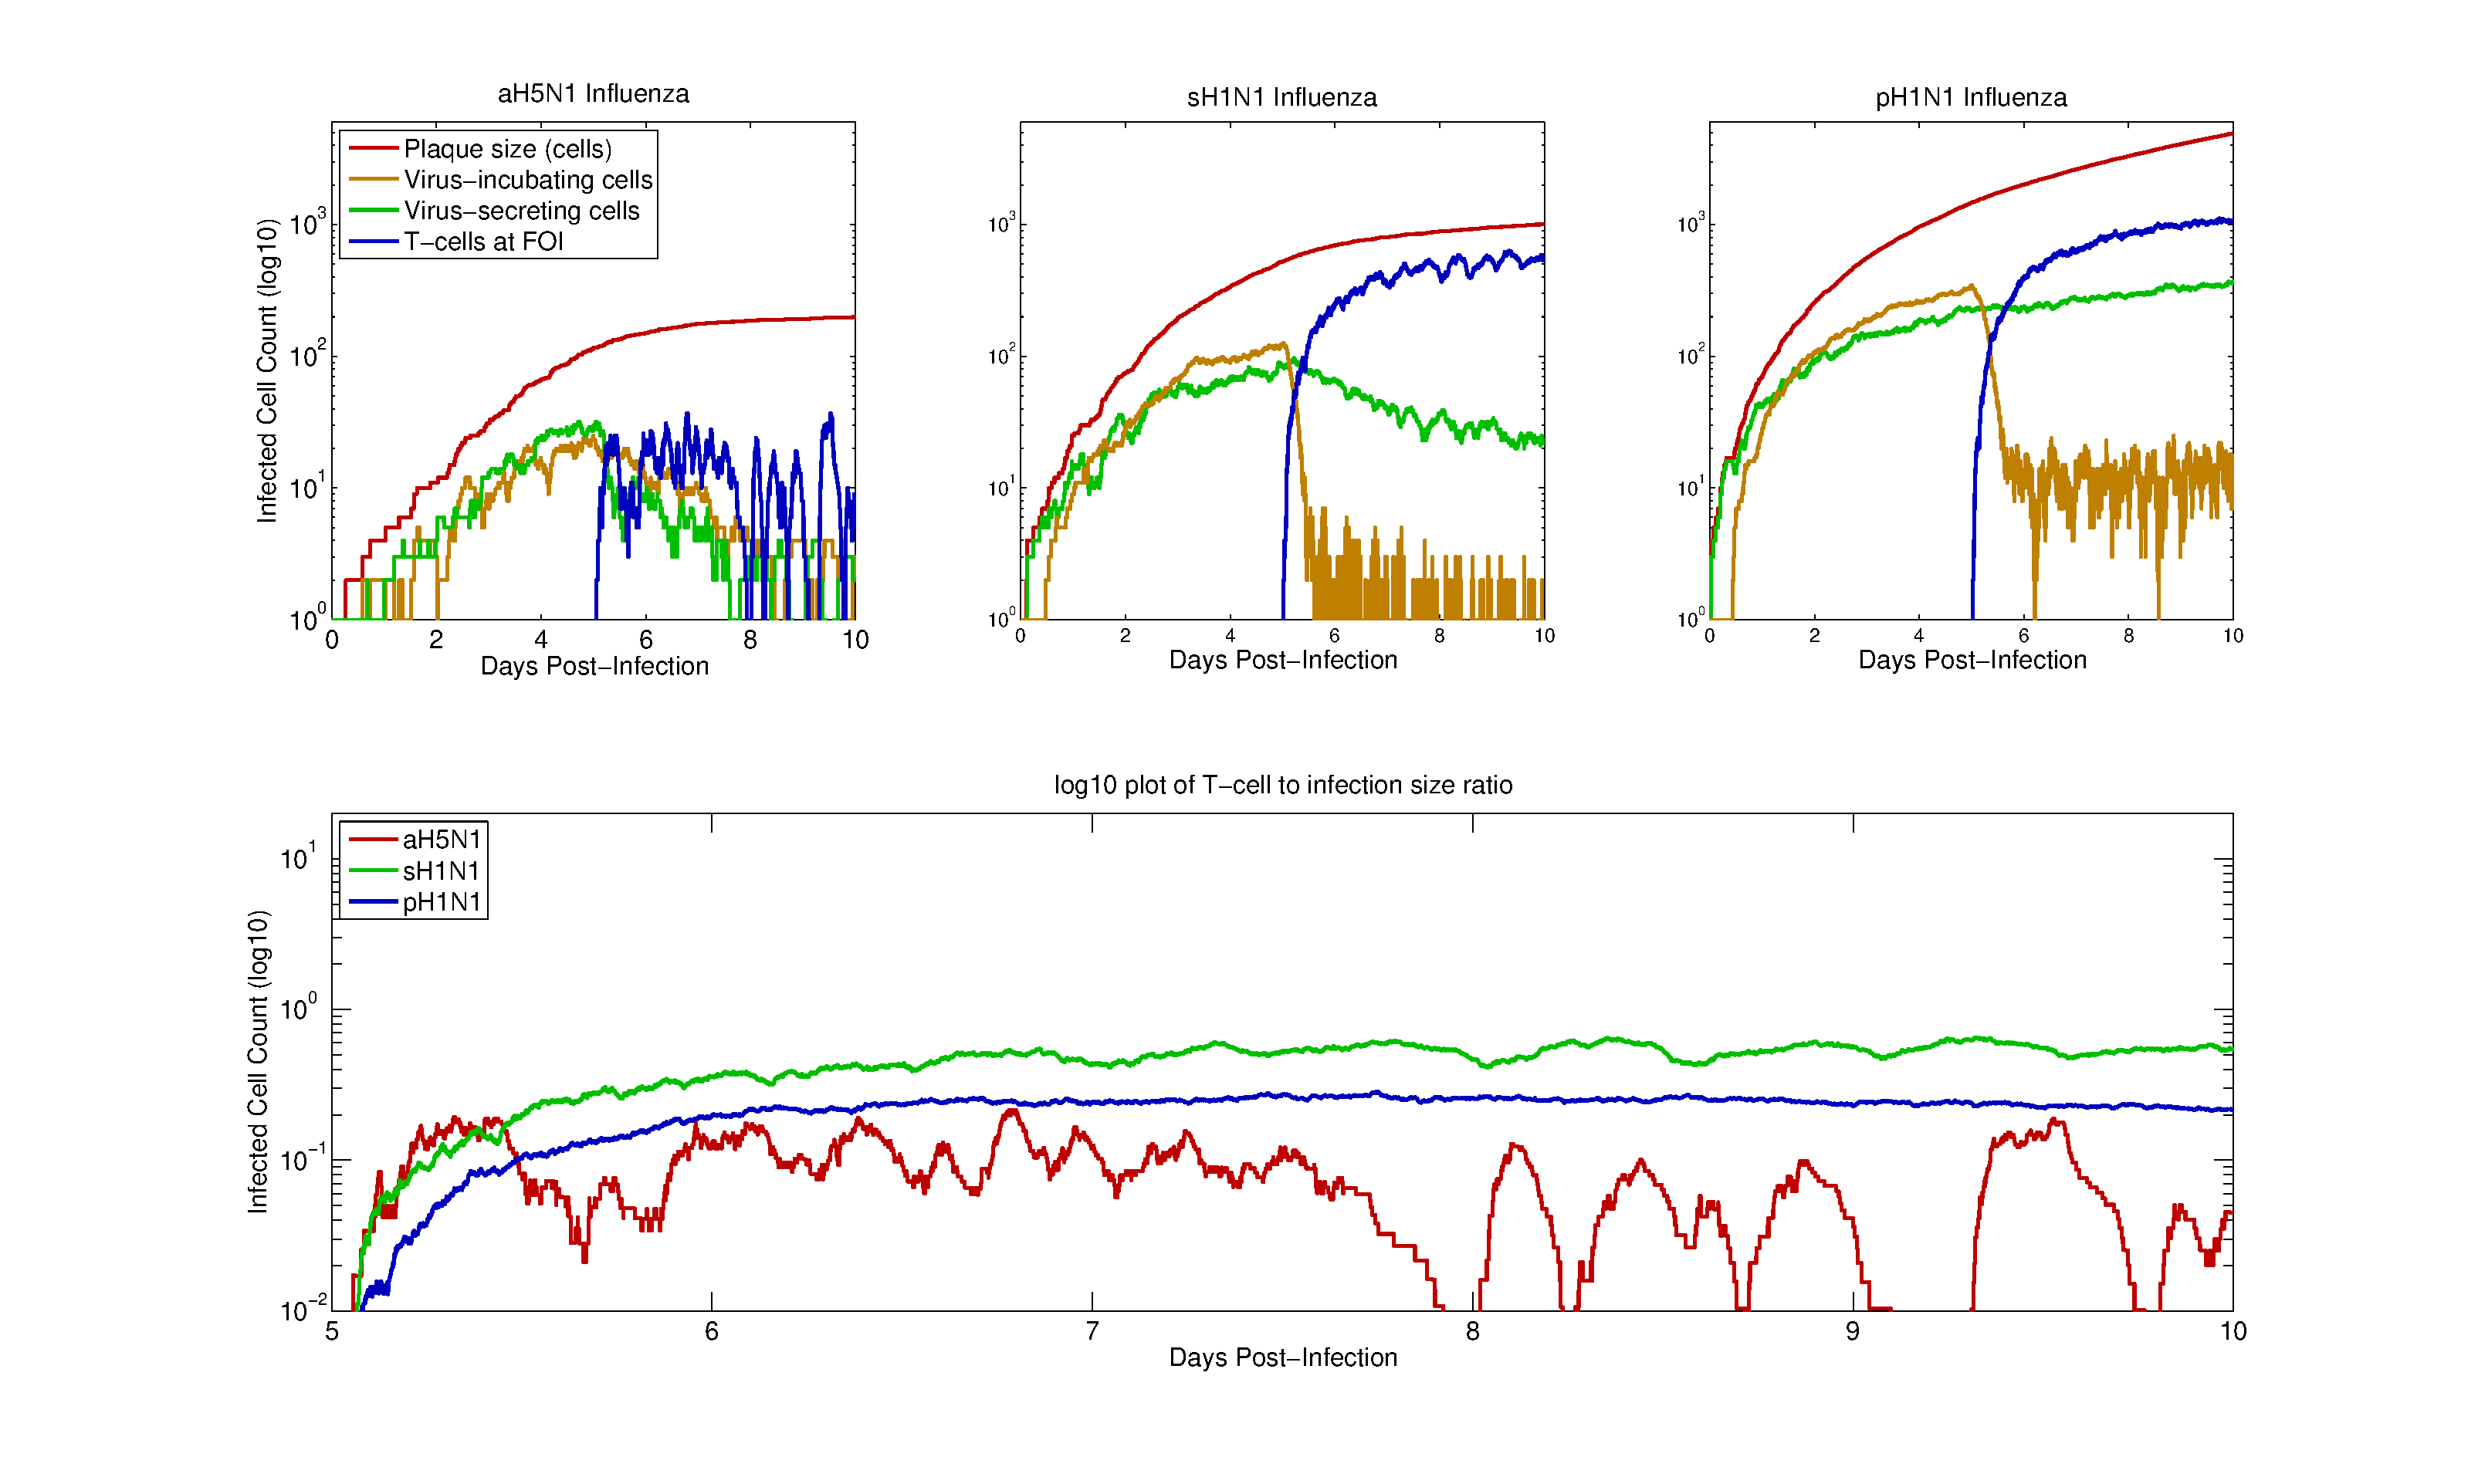
\includegraphics[width=\textwidth]{plaquesize}
 \end{center}
\caption{Comparison of total plaque size (green), number of virus incubating cells (blue), number of virus secreting cells (red), and T-cells (indigo) for the simulated infections of H5N1, sH1N1, and pH1N1.  NOTE TO SELF: Text came out tiny!  Legend is outdated.} 
 \label{fig:plaquesize}
\end{figure}



\section*{Discussion}



\section*{Materials}

Chemokine secretion:  Epithelial cell culture and supernatant collection was performed as described (ref Mitchell 2010).  Briefly, undifferentiated human tracheal epithelial cells (University of Miami) were cultured for 4 weeks to achieve fully differentiated confluent monolayers on collagen-coated transwell inserts, or commercial differentiated human bronchial epithelial cells (EpiAirway Tissue, MatTek Corp., Ashland, MA) used immediately upon receipt, were infected at an MOI of 0.01 with either a seasonal H1N1 virus A/New Caledonia/20/99 (sH1N1), the 2009 H1N1 pandemic strain A/California/04/09 (pH1N1), or an avian H5N1 virus A/Hong Kong/483/97 (aH5N1) derived from a fatal human infection.  Apical fluid for viral secretion, and basal media for chemokine secretion collected before treatment of the monolayer with protease, was collected from previously undisturbed triplicate or quadruplicate wells at 0, 6, 10, 12, 16, 20, 24, 30, 36, 42, 48, and 72 hours after infection, and stored at -80C until assay.  Quantitative viral culture was performed by standard plaque assay.  Quantitative chemokine levels were performed in 30 µl aliquots for a panel of 17 chemokines and cytokines (Luminex Assay®, Luminex Corp.) and reported as ng/mL basal media sampled from a total volume of 4 mL.

% Do NOT remove this, even if you are not including acknowledgments
\section*{Acknowledgments}


%\section*{References}
% The bibtex filename
\bibliography{template}

\section*{Figure Legends}
%\begin{figure}[!ht]
%\begin{center}
%%\includegraphics[width=4in]{figure_name.2.eps}
%\end{center}
%\caption{
%{\bf Bold the first sentence.}  Rest of figure 2  caption.  Caption 
%should be left justified, as specified by the options to the caption 
%package.
%}
%\label{Figure_label}
%\end{figure}


\section*{Tables}
%\begin{table}[!ht]
%\caption{
%\bf{Table title}}
%\begin{tabular}{|c|c|c|}
%table information
%\end{tabular}
%\begin{flushleft}Table caption
%\end{flushleft}
%\label{tab:label}
% \end{table}

\end{document}

